%% Estructura principal para un reporte de Trabajos intersemanales CIRCAE %%
\documentclass[conference]{IEEEtran} %tamaño del papel y el tipo de transcripción que será IEEE
\usepackage[utf8]{inputenc} %el tipo de codificación que incluye símbolos como la tilde
\usepackage[spanish]{babel} % hacemos que nuestro documentación vaya en español
\usepackage{cite} % citas bibliográficas
\usepackage{graphicx} %gráficos, usaremos solo .jpg o .png con estándares que ya veremos
\usepackage{subfigure} %usar subfiguras
\usepackage{url} %agregar direcciones url
\usepackage{amsmath} %expresiones matemáticas
\newtheorem{teor}{Teorema}[section] %definimos la enumeración de Teoremas usando la etiqueta \begin{teor} ... \end{teor} para los ejemplos, podemos darle etiquetas para referenciarlas a lo largo del texto
\newtheorem{ejem}{Ejemplo}[section] %definimos la enumeración de Ejemplos usando la etiqueta \begin{ejem} ... \end{ejem} para los ejemplos, podemos darle etiquetas para referenciarlas a lo largo del texto
\newtheorem{exper}{Experimento}[section] %definimos la enumeración de Ejemplos usando la etiqueta \begin{exper} ... \end{exper} para los Experimentos, podemos darle etiquetas para referenciarlas a lo largo del texto
\usepackage{setspace} %LA usamos para asignar el interlineado
%%%%%%% settings para incluir codigo fuente en cualquier lenguaje
\usepackage{listings} %comenzamos la configuración de nuestras lineas de codigo que se incluirá de ser necesario en el documento
\usepackage[usenames]{color} %seteamos el uso de nombre y color
\definecolor{gray97}{gray}{.97}%definimos nombre y color
\usepackage{textcomp}
\lstset{
		frame=Ltb,
		framerule=1pt,
		framextopmargin=5pt, %margen de arriba
		framexbottommargin=5pt, %margen de abajo
		framexleftmargin= -2pt, %separacion del margen izquierdo
		framesep=2pt,
		rulesep=0.2pt,
		backgroundcolor=\color{gray97},
		rulesepcolor=,
        tabsize=4,
        rulecolor=\color[RGB]{106, 182, 217}, %AZUL
        upquote=true,
        aboveskip={1.5\baselineskip}, %despues de la linea de texto
        columns=fixed,
        showstringspaces=false,
        extendedchars=true,
        breaklines=true,
        prebreak = \raisebox{0ex}[0ex][0ex]{\ensuremath{\hookleftarrow}},
        showtabs=false,
        showspaces=false,
        showstringspaces=false,
        basicstyle=\scriptsize\ttfamily\color[RGB]{39, 100, 46}, %Numeros de lineas, simbolos, puntos y coma y demas
        identifierstyle=\ttfamily\color[RGB]{56, 140, 189}, %variables
        commentstyle=\color[RGB]{62, 179, 101}, %comentarios
        stringstyle=\color[RGB]{247, 165, 42}, %impresiones
        keywordstyle=\bfseries\color[RGB]{237, 118, 150}, %funciones
        %
		numbers=left,
		numbersep=-7pt, %separacion del numero
		numberstyle=\tiny,
		numberfirstline = false,
		breaklines=true,
		}
\usepackage{graphicx}
\usepackage[colorinlistoftodos]{todonotes}
\usepackage{array}
\usepackage{fixltx2e}
\usepackage{float}
%%%%%%%
\providecommand{\keywords}[1]{\textbf{\textit{Términos Clave---}} #1}

\begin{document}
\spacing{0.9} %definimos un interlineado de 0.9 para todo el documento

\title{Diseño de fuentes de corrientes para amplificadores diferenciales con Nanotubos de Carbono - CNT {\footnotesize \textsuperscript{*}Recopilación bibliográfica de amplificadores diferenciales}}

\author{
	\IEEEauthorblockN{1\textsuperscript{st} Edison Abado Ancco}
	\IEEEauthorblockA{\textit{Escuela profesional de Ingeniería Electrónica} \\
		\textit{Universidad Nacional de San Antonio Abad del Cusco}\\
		145012@unsaac.edu.pe}
	
	\and
	\IEEEauthorblockN{2\textsuperscript{nd} Wilmer Condori Olivera}
	\IEEEauthorblockA{\textit{Escuela profesional de Ingeniería Electrónica} \\
		\textit{Universidad Nacional de San Antonio Abad del Cusco}\\
		182962@unsaac.edu.pe}
	\and
	\IEEEauthorblockN{3\textsuperscript{rd} Kevin Cuba Arenaza}
	\IEEEauthorblockA{\textit{Escuela profesional de Ingeniería Electrónica} \\
		\textit{Universidad Nacional de San Antonio Abad del Cusco}\\
		182963@unsaac.edu.pe}
	\and
	\IEEEauthorblockN{4\textsuperscript{th} Joseph Garfias Quispe}
	\IEEEauthorblockA{\textit{Escuela profesional de Ingeniería Electrónica} \\
		\textit{Universidad Nacional de San Antonio Abad del Cusco}\\
		182966@unsaac.edu.pe}
	\and
	\IEEEauthorblockN{5\textsuperscript{th} Roly S. Gutierrez Benito}
	\IEEEauthorblockA{\textit{Escuela profesional de Ingeniería Electrónica} \\
		\textit{Universidad Nacional de San Antonio Abad del Cusco}\\
		182967@unsaac.edu.pe}
	
}




\markboth{CIRCAE INFORME \today -G1-P3-005}{} % Codigo del informe que corresponde a: - numero de grupo con la G antepuesta - numero de proyecto con la P antepuesta | número de informe
\maketitle


\begin{abstract}
	El trabajo bibliográfico presente, recompila información de nuevos componentes para la mejora 
	de los diseños de los dispositivos analógicos y digitales, empleando transistores de efecto de campo de nanotubos de carbono de tipo n (CNTFET - CNFET), donde se observo que existe mejora sustancial en la ganancia de voltaje, reducción de potencia consumida 
	en el diseño de los amplificadores diferenciales
	y otras mediciones en comparación con otros amplificadores diferenciales - DA convencionales, estas mejoras estan atribuidas a las propiedades de los nanotubos de carbono.\\
	
	\keywords{\textbf{Nanotubos de carbono - CNT, transistores CNTFET, amplificadores diferenciales - DA, ganancia, ancho de banda.}}
\end{abstract}

\section{Introducción}

Cada año se busca mejorar el rendimiento y velocidad en los aparatos electrónicos, ya sea innovando con nuevas tecnologías o rediseñando la tecnología existente; siguiendo la ley de Gordon Moore, este establecía que el número de transistores (elementos electrónicos semiconductores) en un microprocesador se duplicaría cada dos años y que los ordenadores, los componentes que funcionan en ordenadores y la potencia informática se volverían más pequeños y rápidos, a medida que los transistores de los circuitos integrados se vuelven más eficientes.
Una confirmación de que esta ley se sigue cumpliendo es el estudio y diseño de los nanotubos de carbono aplicados en los transistores, siendo el principal punto de estudio en el presente artículo, que a diferencia de los transistores CMOS convencionales estos operan a una mayor velocidad y eficiencia, además se libra de la influencia de los parámetros térmicos haciendo su diseño e implementación más sencilla. Sin embrago, este material presenta algunas complicaciones de las cuales se hablará más adelante en este artículo.


\section{FET de Nanotubos de Carbono}
Las necesidades de eficiencia nos llevan a buscar nuevas maneras de realizar tareas con el fin de aumentar la eficiencia, partiendo de ello se tiene a un dispositivo electrónico cuya composición se gestó en 1991 por Sumio Ijima (un nanotubo multicapa) y en 1993 con Donal Bethude que produjo nanotubos de Carbono de una sola capa.

Desde entonces, se fueron desarrollando nanotubos de carbono para diferentes aplicaciones, entre ellas, la que más nos interesa, los nanotubos de carbono para aplicaciones de semiconductores, para ser más específicos, el CNFET o CNTFET (Carbon Nanotube FET) cuyo diámetro de circunferencia va desde $<1nm$ hasta $50nm$ \cite{DesignandSimulationofCarbon2021} para aplicaciones de nuestro interés.

El esquema de un CNFET (figura \ref{img11}) es parecido al del FETs a base silicio, requiere de tres pines, y también la compuerta (Gate) controla el flujo de corriente a través del canal. El switching de la compuerta habilita  la corriente del canal \cite{PerformanceAnalysisofClassical2018}. La construcción se muestra en la figura \ref{img13}. 

\begin{figure}
	\centering
	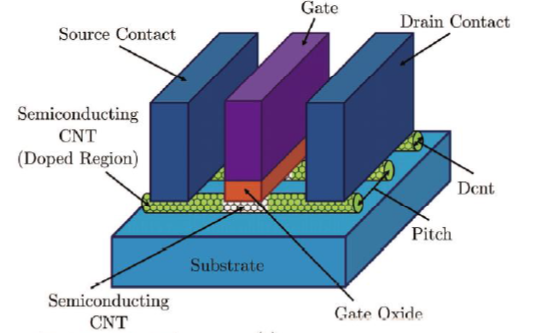
\includegraphics[width=6cm]{IMAGENES/img11}
	\caption{Diseño de un CNFET como un MOSFET \cite{DesignofanovelternarySRAM2017}}
	\label{img11}
\end{figure}




\subsection{Clasificación de nanotubos de carbono}
Existen 3 tipos: el CNFET de barrera de Shottky, CNFET de tunelamiento banda-a-banda y el CNFET como-MOSFET \cite{DesignofanovelternarySRAM2017}. Otra clasificación se da por el tipo de distribución de las celdas hexagonales que presentan estos modelos.

\begin{figure}
	\centering
	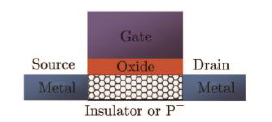
\includegraphics[scale=0.7]{IMAGENES/img16}
	\caption{CNFET de barrera de Shottky \cite{DesignofanovelternarySRAM2017}.}
	\label{img16}
\end{figure}

\begin{figure}
	\centering
	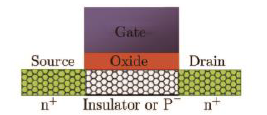
\includegraphics[scale=0.7]{IMAGENES/img17}
	\caption{CNFET de tunelamiento banda-a-banda \cite{DesignofanovelternarySRAM2017}.}
	\label{img17}
\end{figure}

\begin{figure}
	\centering
	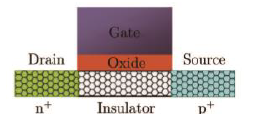
\includegraphics[scale=0.7]{IMAGENES/img18}
	\caption{CNFET como-MOSFET. \cite{DesignofanovelternarySRAM2017}.}
	\label{img18}
\end{figure}

\begin{enumerate}
	\item Nanotubo de una sola capa (SWNT), el valor de su diámetro varia de $1nm$ a pocos micrometros basado en la quiralidad que presenta\\
	\item Nanotubo Multicapa (MWNT), son más costosos y se encuentran en los cables coaxiales, su diámetro varia de $5nm$ \\
	\item Nanotubo Mixto, este modelo varia de diametro entre los $2nm$ a $5nm$
\end{enumerate}
	
	\begin{figure}
		\centering
		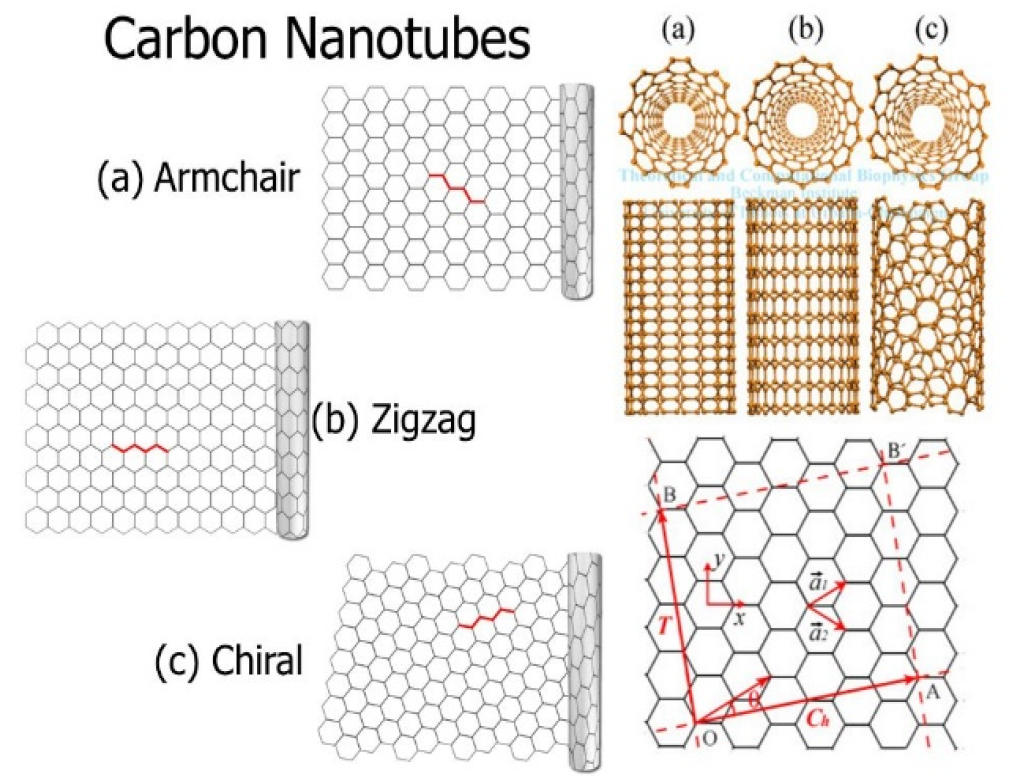
\includegraphics[width=6cm]{IMAGENES/img12}
		\caption{Los principios de construcción del CNT de planchas de grafeno \cite{PerformanceAnalysisofClassical2018} .}
		\label{img12}
	\end{figure}
	


\begin{figure}
	\centering
	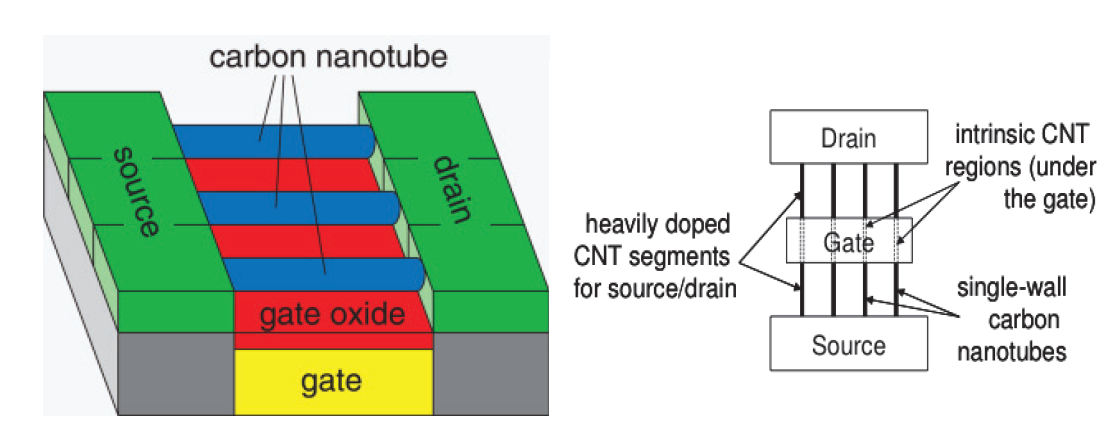
\includegraphics[width=8cm,height=4cm]{IMAGENES/img13}
	\caption{Estructura del CNFET \cite{Performanceinvestigationofemerging2016}.}
	\label{img13}
\end{figure}

%%%%%%%%%%%%%%%%%%%%%%%
% mencionar imagenes %%
% EDISON%%%%%%%%%%%%%%%


\section{Comparación de eficiencia energética}

\subsection{Tecnología de 7nm por nodo}

Mediciones para un chip multi nucleo de OpenSPARC T2 muestra que este CNFET 9 veces más beneficio que los de Si/SiGe, pueden operar 3 veces más rápido en frecuencia de reloj y consumen 3 veces menos energía por ciclo de reloj.

\begin{figure}
	\centering
	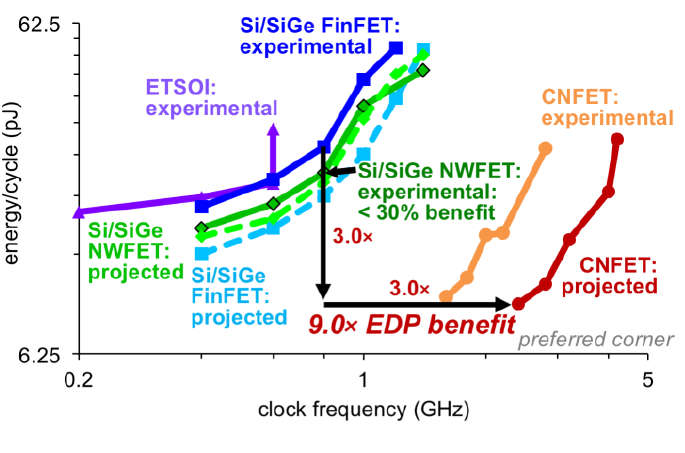
\includegraphics[width=8cm]{IMAGENES/img14}
	\caption{Comparación de otros dispositivos con CNFET de 5nm \cite{UnderstandingEnergyEfficiency2018} .}
	\label{img14}
\end{figure}

\subsection{Tecnología de 5nm por nodo}

Mediciones para un nucleo de procesador comercial de 32 bits muestra que este CNFET 9.3 veces más beneficio que los de Si/SiGe, pueden operar 3.1 veces más rápido en frecuencia de reloj y consumen 3 veces menos energía por ciclo de reloj.

\begin{figure}
	\centering
	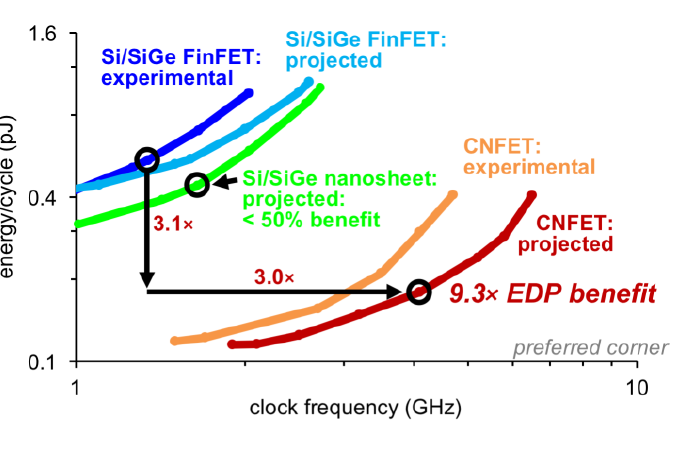
\includegraphics[width=8cm]{IMAGENES/img15}
	\caption{Comparación de otros dispositivos con CNFET de 7nm \cite{UnderstandingEnergyEfficiency2018} .}
	\label{img15}
\end{figure}

Estas mediciones muestran que mientras más pequeño el nodo de CNFET, se mejora la eficiencia. Además, la ganancia intrínseca aumenta mientras más se reduce el tamaño \cite{CarbonNanotubeCMOS2019} en comparación a los de Silicio que al aumentar tamaño disminuye su ganancia intrínseca (figura \ref{img19}).



\begin{figure}
	\centering
	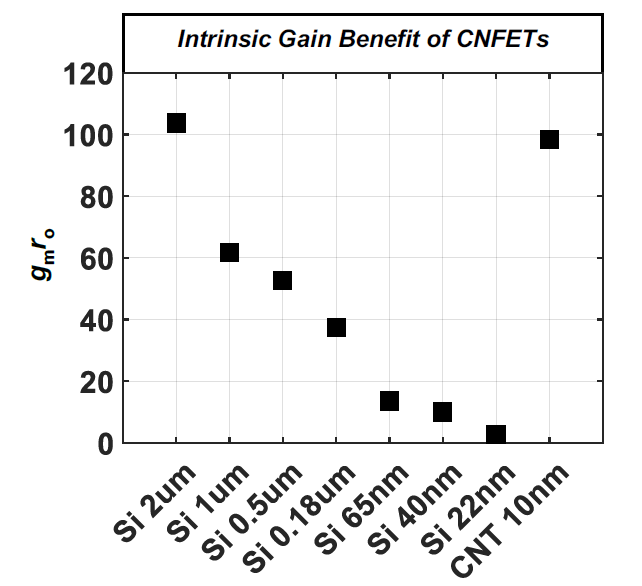
\includegraphics[width=8cm]{IMAGENES/img19}
	\caption{Comparación de otros dispositivos con CNFET de 7nm \cite{UnderstandingEnergyEfficiency2018} .}
	\label{img19}
\end{figure}



%----------------- Diseño de fuentes de corrientes ---------------------
\section{Criterios de diseño de fuentes de corriente}
La parte primordial de los amplificadores operacionales son los DA (Differential amplifier), ya que este amplifica la diferencia de dos entradas de voltaje. Estos están elaborados con tecnologías CMOS y los BJT, que con el tiempo se observó las deficiencias que presenta.
\begin{itemize}
	\item Elevado consumo de energía
	\item Velocidad de tecnología en los bipolares es menor
	\item Los MOSFET en escalas de nano presenta limitaciones
\end{itemize}

En ese sentido se hace uso de los CNTFET (transistor de efecto de campo de nanotubos de carbono) que son los nuevas herramientas del futuro para los dispositivos electrónicos.\\
Como menciona \cite{Akhoon}, CNTFET es un dispositivo prometedor y se puede utilizar para extender la validez de la ley más conocida de Gordan Moore. Se ha encontrado que el CNTFET intrínseco tiene Características $CV/I \sim 13$ veces más altas que las de un convencional $n-MOSFET$, el transistor de efecto de campo de nanotubos de carbono (CNFET) es una excelente alternativa a un transistor a granel tradicional para bajo consumo de energía y alto rendimiento, según \cite{Liu}

\begin{itemize}
	\item Reducción de potencia consumida 
	\item Alta velocidad de procesamiento
	\item Eficiencia en los circuitos integrados 
	\item Gran capacidad de conducción eléctrica 
	\item Alta resistencia a la tracción
	\item Conductividad térmica
\end{itemize}

Son laminas de grafeno enrollados en tubos, que presentan características: 

\begin{itemize}
	\item Eléctricas
	\item Mecánicas
	\item Semiconductoras
	\item Prop. optoelectrónicas
\end{itemize}

De acuerdo a la figura \ref{img12}, podemos observar la estructura interna de los nanotubos, lo cual nos proporciona las propiedades mencionadas, que dependerán del diámetro, la distancia entre los nanotubos y el voltaje umbral con el que trabaja.

\textbf{Diámetro de los nanotubos}:
\begin{equation}
	D_{CNT} =  \frac{\sqrt{3}a_0}{\pi}\sqrt{n^2 + m^2 + mn}
\end{equation}
Donde:
\begin{itemize}
	\item n,m son los valores de vectores de quiralidad del nanotubo
	\item $a_0$ distancia interatómica entre cada átomo de carbono
\end{itemize}

\textbf{Voltaje umbral}
\begin{equation}
	V_{th}\approx \frac{E_g}{2e} = \frac{\sqrt{3}}{3}\frac{a V_{\pi}}{eD_{CNT}}
\end{equation}
\begin{itemize}
	\item $a= 2.49A$, distancia de carbono a átomo de carbono
	\item $V_{\pi} = 3.033eV$ energía de enlace del carbono
	\item $e$, es el valor de la carga del electrón
\end{itemize}

\textbf{Ancho de banda}
\begin{equation}
	W = (N-1)S+D_{CNT}
\end{equation}
\begin{itemize}
	\item N, números de CNTS
	\item S, es la distancia entre el centro de dos CNTs (factor importante para el diseño)
\end{itemize}
\textbf{\textit{La influencia de varios parámetros de $CNTFET$, N, S y $D_{CNT}$}}

\begin{figure}
	\centering
	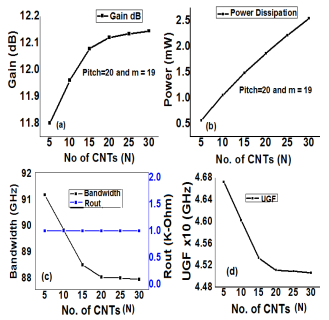
\includegraphics[scale=0.6]{IMAGENES/4.PNG}
	\caption{Variación de (a) Ganancia de corriente (b) Disipación de potencia (c) Ancho de banda (d) Frecuencia de ganancia unitaria con N en la propuesta basada en CNT-DA\cite{Akhoon}}
\end{figure}




\begin{figure}
	\centering
	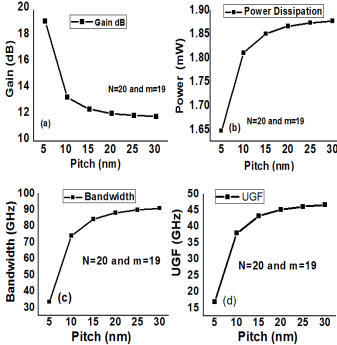
\includegraphics[scale=0.6]{IMAGENES/5.PNG}
	\caption{Variación de (a) ganancia de corriente (b) Disipación de potencia (c) Ancho de banda (d) Frecuencia de ganancia unitaria con respecto al tono de CNT-DA \cite{Akhoon}}
\end{figure}




\begin{figure}
	\centering
	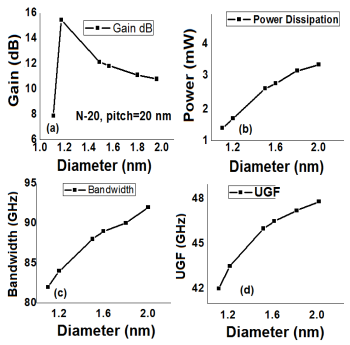
\includegraphics[scale=0.6]{IMAGENES/6.PNG}
	\caption{Variación de (a) Ganancia (b) Disipación de potencia (c) Ancho de banda (d) Frecuencia de ganancia unitaria con respecto al diámetro de CNT-DA \cite{Akhoon}}
\end{figure}


%-------------------- Fuentes de corrientes --------------------------


\section{Fuentes de corrientes}
Algunas fuentes de corrientes
\begin{itemize}
	\item Fuente de corriente constante cascode
	\item Fuente de corriente constante con FET(Mosfet)
\end{itemize}


\subsection{Fuente de corriente constante cascode}

Una forma de eliminar la disparidad de $V_{DS}$ es usar la configuración cascode:
\begin{figure}
	\centering
	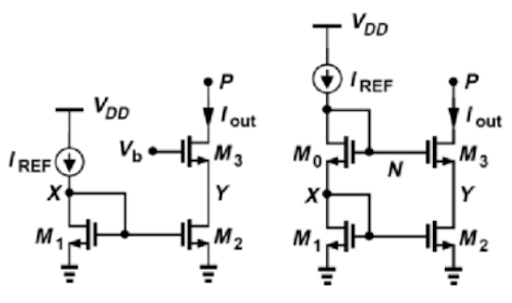
\includegraphics[scale=0.5]{IMAGENES/image3.png}
	\caption{Fuente de corriente en cascode}
	\label{image3}
\end{figure}



$V_{DD}$ tal que $V_X = V_Y$
$$\dfrac{\left(\dfrac{W}{L}\right)_3}
{\left(\dfrac{W}{L}\right)_0} = 
\dfrac{\left(\dfrac{W}{L}\right)_2}
{\left(\dfrac{W}{L}\right)_1}$$ 

donde
\begin{center}
	\hspace{-5mm}W: ancho de puerta\\
	L: longitud de la puerta
\end{center}



\begin{align}
	V_{P_{min}} &= V_{DS_{sat_{2}}} + V_{DS_{sat_3}} \\
	V_{P_{min}} &= (V_{GS_0} - V_{TH_0}) + (V_{GS_1} - V_{TH_1}) \\
	V_{P_{min}} &= 2V_{DS_{sat}} + V_{TH_3} = 2V_{OD} + V_{TH} \\
\end{align}
Dimensionando correctamente los transistores logramos que $M_3$
absorba las variaciones de $V_P$ y mantenga $V_X = VY$.\newline

Por debajo de la tensión mínima de salida, $M_3$ ya no puede 
absorber las diferencias de $V_{DS}$ y $V_B$ y será distinto a 
$V_A$, volviendo a los problemas de espejo simple. Para tensiones
muy bajas, la resistencia de salida se degrada.

\begin{figure}
	\centering
	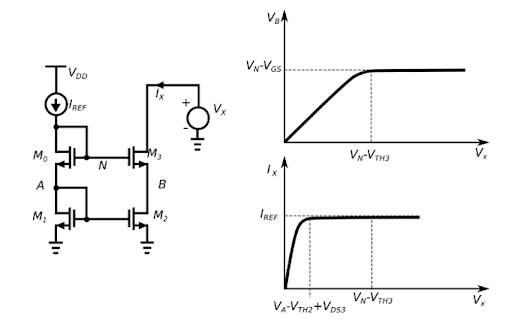
\includegraphics[scale=0.5]{IMAGENES/image4.png}
	\caption{Gráfica de la ganancia de voltaje con fuente Widlar}
\end{figure}


\subsection{Fuente con FET}


\begin{itemize}
	\item El par diferencial básico consta de dos MOSFET de enriquecimiento acoplados ($Q_1$ y $Q_2$), polarizados con una fuente de corriente constante; esta ultima suele ser una configuración de espejo de corriente similar a la utilizada con BJT’s. desde luego se supone que el circuito de carga es tal que los dos MOSFET que conforman el par, se encuentran operando en la región de saturación.
	\item El MOSFET es frecuentemente usado como amplificador de potencia y ofrece como ventaja una resistencia de entrada alta, prácticamente infinita en la compuerta y una corriente de polarización de entrada cai cero.
	\item Existen dos razones fundamentales por las cuales se prefieren los amplificadores diferenciales sobre los de un solo extremo: son sensibles a la interferencia y no necesitan capacitores de paso y acoplamiento.
\end{itemize}

\begin{figure}
	\centering
	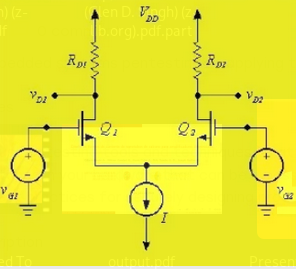
\includegraphics[width=5cm]{IMAGENES/image5.png}
	\caption{Amplificador diferencial con FETs}
\end{figure}




\section{Conclusiones}

\begin{itemize}
	\item Las fuentes de corrientes   basados en nanotubos de carbono y FETs tienen ventajas por encima que los BJTs: no dependen de hie, por ende no se verán afectados por la temperatura.
	
	\item Las fuentes de corrientes se usan en los amplificadores de corriente como un elemento de amplificador, ya que fijará un valor constante para el punto de operación del amplificador diferencial.
	
	\item Con una tensión de alimentación de 0,4 voltios, la corriente que fluye a través del transistor de nanotubos de carbono es mayor que la que obtendrían los mejores transistores CMOS.
	
	\item Los CNTFET presentan una precisión referencia de banda prohibida con una salida nominal de $500 mV$, $6,8$ coeficiente de temperatura $ppm/°C$, sensibilidad de línea de $±2,25 mV/V$
	y se presenta una disipación de potencia de $26 µW$. 
	
	
	\item 
\end{itemize}



 

%%%%%%%%%%%%%%%%%%%%%%%%%%%%%%%%%%%%%%%%%%%%%%%
%%%%%
%%%%%   BIBLIOGRAFÍA     %%%%%%%%%%%%%%%%%%%%%%
%%%%%
%%%%%%%%%%%%%%%%%%%%%%%%%%%%%%%%%%%%%%%%%%%%%%%

\bibliographystyle{ieeetr}
\bibliography{bibliografia}

\end{document}
